%    \chapter{Pilotage du projet}
\section{Cycle de vie itératif}
Pour développer l’Interpréteur LIR, le modèle de cycle de vie itératif a été
choisi. Ce modèle de développement de logiciel, rappelons-le, consiste en une
succession de cycles de spécification, de conception, de réalisation et de
tests, le but est d’enrichir et de « remodeler » des prototypes du logiciel
successifs. Par conséquent, une version du logiciel sera un « dernier
prototype ».
\\Si le choix de modèle de cycle de vie s'est porté sur le modèle itératif,
c'est parce qu'il s'agit d'un modèle "réaliste" et possible à mettre en place
dans le cadre des projets tuteurés :

\begin{itemize}
    \item Une limitation de "l'effet tunnel" pour une meilleure dynamique et motivation des équipes (MOA et MOE).
    \item Une meilleure acceptation des changements grâce aux prototypes.
    \item Une meilleure gestion des risques.
    \item Est adapté pour une équipe de cinq personnes polyvalentes.
    \item Le principe d'itérations où seules les fonctionnalités nécessaires sont spécifiées en détail en début d'itération ce qui permet une évolution du besoin.
\end{itemize}

\section{Estimation initiale}
En se focalisant sur un développement de type Organic d'une taille attendue
de 2000 lignes de code (2KLOC), le projet nécessite de base un effort de 4,97
mois.homme répartis sur une durée de 4.60 mois. Cette estimation se base sur
une équipe d'un seul développeur.

\'{E}tant donné que notre équipe se constitue de 5 personnes, il nous suffit
d'adapter cette estimation en divisant l'effort par le nombre de membres. Nous
obtenons ainsi un effort de 0, 99 mois de 20 jours. Notre contexte de travail
étant toutefois différent de celui d'une entreprise (pas d'horaires fixes,
travail les jours fériés,...), il nous a paru plus judicieux de convertir
notre estimation vers un format plus réaliste.

En considérant une durée de deux heures par journée de travail par personne,
nous arrivons à un total de 10 heures quotidiennes, soit un total de
200 heures hebdomadaires. Nous conservons la durée de 20 jours par mois pour
pallier les indisponibilités de chacun. La durée totale du projet est donc
estimée à 0,99 mois ou 200 heures de travail total, soit 40 heures.homme.

\section{Planification prévisionnelle initiale}
Le développement de l'interpréteur LIR suivant un cycle de vie itératif,
nous agréé avec la MOA de trois itérations, avec à l'issue de chacune la
livraison d'un prototype fonctionnel ou, dans le cas de la dernière itération,
du programme complet.

Pour la première itération, nous avons convenu de livrer un prototype
incluant les mécanismes de base du fonctionnement des commandes et instructions.
Cette première mouture de l'interpréteur Doit être en mesure d'analyser son
entrée standard, d'affecter des variables de type chaîne à son contexte
d'exécution et de reconnaître les expressions sur les chaînes de caractères.
Le contexte pourra être réinitialisé.
Enfin, ce prototype devra afficher les variables déclarées, afficher le
résultat d'une expression de type chaîne, et être en mesure
mettre fin à la session.

Lors de la seconde itération, notre prototype devra, en plus des fonctionnalités
sus-mentionnées, incorporer l'affectation de variables de type entier
et l'arithmétique entière sur les expressions. L'interpréteur, à ce stade du
développement, devra être en mesure de reconnaître des étiquettes de ligne de
code et garder en mémoire centrale un programme pour pouvoir ensuite l'afficher ou
l'exécuter. Il doit également être en mesure de supprimer des lignes de code dans
le programme global. Il sera également possible à l'utilisateur de saisir puis
d'affecter la valeur d'une variable via l'entrée standard ou d'effectuer des sauts
non-conditionnels dans un programme.

Enfin, le programme final de la troisième itération pourra lire et écrire des
programmes vers et depuis des fichiers. Il sera possible au programmeur d'effectuer
des sauts conditionnels. Seront livrés avec ce prototype final ce plan de projet
complété, ainsi que le manuel d'utilisateur de l'interpréteur LIR. Le prototype
final devra pouvoir être lancé à partir d'un fichier exécutable.

\section{Durée et ordonnancement des principales tâches et itérations}

Afin d'avoir un interpréteur LIR fonctionnel, nous avons identifié un jeu de
tâches critiques devant être remplies à chaque itération. Ainsi, pour la
présentation du premier prototype, devront être implémentés et testés les
littéraux, les idendificateurs, les variables, le contexte d'exécution, les
commandes et instructions, et l'analyseur lexicale.

Lors de la deuxième itération, devront être traités en priorité la gestion des
étiquettes et l'implémentation de programmes à stocker en mémoire. Enfin,
l'analyseur devra prendre en compte cette nouvelle fonctionnalité et référencer
le programme global de la session.

Pour finir, la troisième itération consistera à rajouter la possibilité au
programmeur d'effectuer des sauts conditionnels. Pour ce faire, les conditions
devront être traitées sous la forme d'une expression booléenne simple. Cela
implique donc la création d'un littéral de type booléen, non accessible directement
au programmeur dans cette version de l'interpréteur (le programmeur ne pourra donc
pas créer de variable de type Booléen). La troisième itération se terminera par
la revue du code et des jeux de tests, l'édition du manuel utilisateur, ainsi que
la complétion du dossier technique.

\section{Identification des premiers jalons}
Chacun des prototypes de l'interpréteur LIR devant être livré à l'issue de chaque
itération, nous pouvons donc en déduire les premiers jalons ci-dessous. La date de
soutenance du projet, quand à elle, nous sera précisée à une date ultérieure à
la rédaction de ce plan. Nous ne pouvons donc en donner qu'une estimation.

\begin{itemize}
    \item Premier entretien MOA / MOE et lancement du projet :
          jeudi 8 avril
    \item Livraison du premier prototype : lundi 10 mai
    \item Livraison du deuxième prototype : mercredi 19 mai
    \item Livraison du prototype final : Vendredi 28 mai
    \item Soutenance du projet : entre le 9 et je 11 juin
\end{itemize}

\section{Calendrier prévisionnel}
\`{A} partir des dates citées plus haut, nous pouvons donc en déduire le
calendrier prévisionnel suivant. Les comités de pilotage ont été convenus avec
la maîtrise d'ouvrage afin de conserver un suivi le plus régulier possible sur
l'avancement du développement.
\begin{itemize}
    \item Première itération : du 3 au 10 mai
    \item Deuxième itération : du 11 au 19 mai
    \item Comité de pilotage : mardi 18 mai
    \item Troisième itération : du 20 au 28 mai
    \item Comité de pilotage : mercredi 26 mai
    \item Remise du dossier technique : mardi 8 juin
\end{itemize}

\section{Organisation des réunions projets et comités de pilotage}
Comme mentionné, les comités de pilotage se tiennent entre deux livraisons
afin de faire le point sur l'avancement de l'itération. Compte tenu des restrictions
sanitaires imposées au cours de la crise due à la Covid-19, nous devrons adapter
ces réunions aux modalités de présence imposées par l'IUT de Rodez. Selon la
semaine, certains membres de l'équipe devront y assister en visio-conférence.

Les réunions de projet, quand à elles, se tiennent à chaque fois qu'un ensemble de
tâches est complété pour mettre en commun le travail effectué et faire le point sur
les difficultés techniques rencontrées et la répartition des ressources sur les
tâches restantes (nous privilégions en effet le travail en binôme et faisons en
sorte que chaque membre de l'équipe ait l'occasion de travailler au moins une fois
avec tous les autres).

\section{Suivi du projet pour la première itération}

\subsection{Planification et ordonnancement des tâches}
Au tâches déjà spécifiées dans la section \hyperref{Durée et ordonnancement des principales tâches et itérations}, nous souhaiterions ajouter quelques
fonctionnalités de base de l'interpréteur LIR. La planification de cette itération
comprend donc l'implémentation et le test des commandes \verb|defs|, \verb|debut|
et \verb|fin|, ainsi que des instructions \verb|affiche| et \verb|var|.

Ce premier prototype fonctionnera uniquement avec des données de type chaîne
de caractère. Cela implique donc l'ajout d'identificateurs, de constantes
littérales et d'expressions correspondants.

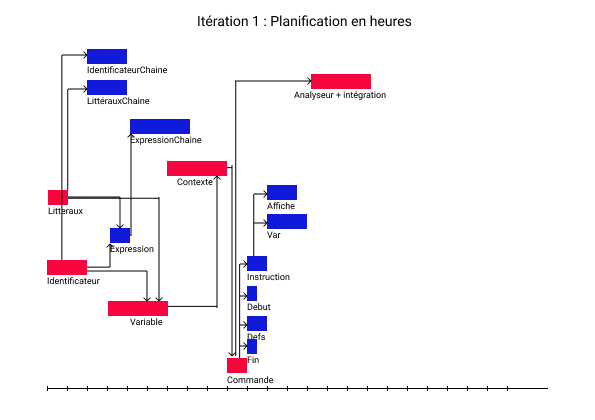
\includegraphics[scale=0.75]{fichiers/planification/iteration1/iteration1Planif.png}

Le diagramme de planification de l'itération 1 suggère un total de 27 heures de
travail, soit l'équivalent de 10 jours.homme. En raison du nombre limité de
ressources de travail, toutes les tâches, notamment les instructions et commandes,
ne pourront être réalisées en concomitance. Certaines devront donc se voir
repousser le temps qu'un binôme se libère.



\subsection{Suivi d’avancement et mesure des écarts par rapport au prévisionnel}

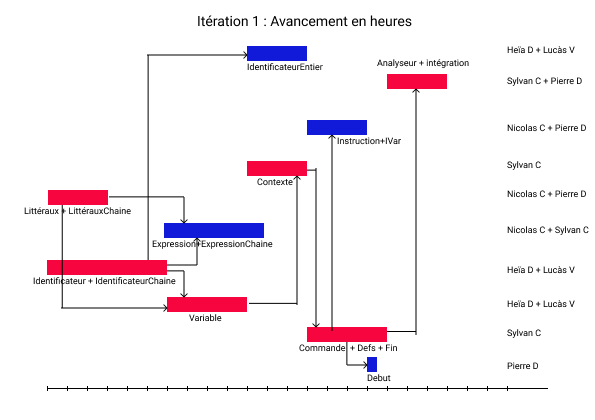
\includegraphics[scale=0.75]{fichiers/planification/iteration1/iteration1Avancement.png}

\`{A} l'issue de cette première itération, nous constatons un volume de travail
total de 35 heures, soit 8 heures ou 4 jours.homme de plus que ce qui était
estimé. Cet écart s'explique d'une part dans une estimation trop optimiste de la
durée des tests unitaires d'une part et un manque d'habitude à travailler en
binôme d'autre part. Cette itération portant sur des aspect structurels importants
de l'interpréteur, il nous sera plus aisé à l'avenir de rajouter les commandes
et instructions.

%    \subsection{Synthèse par "tableau de bord"}

\subsection{Résultats des tests et recette de prototype de la période}

%    \subsection{Résultats des revues/suivis/contrôles qualité de la période}

\subsection{Identification des principaux écarts et problèmes constatés, solutions possibles}
\`{A} l'issue de cette première période, nous avons pu livrer un prototype
fonctionnel et ce malgré des difficultés liées à la conception. En revanche,
l'instruction \verb|affiche|, initialement prévue pour cette itération, n'a
pas été implémentée, faute de temps et de ressources disponibles, et a donc été
reportée à l'itération suivante. Cette instruction n'étant pas critique pour
le fonctionnement de l'application, nous pouvons donc considérer la gravité
de ce retard comme minime.

\subsection{Propositions de modification de la planification prévisionnelle pour tenir compte des corrections à apporter}
Afin de tenir compte de ce léger retard, nous rajouterons l'implémentation de
l'instruction \verb|affiche| aux tâches à réaliser pour la prochaine itération.
En plus des programmes, et l'adaptation de l'analyseur à interagir avec, nous en
profiterons pour implémenter un maximum de fonctionnalités, ce qui nous permettra
de rattraper le léger retard pris sur la planification originelle.

Nous laisserons toutefois l'instruction \verb|si..vaen| et les expressions
conditionnelles qu'elle utilise de côté. En effet, ces dernières nécessiteront
probablement un \emph{refactoring} de la classe Expression et de ses dérivées.

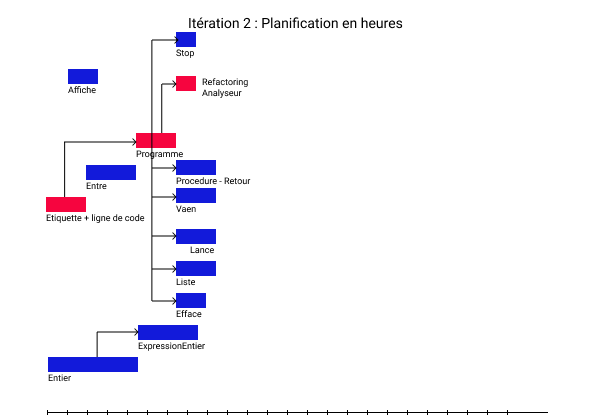
\includegraphics[scale=0.75]{fichiers/planification/iteration2/iteration2Planif.png}

En suivant la planification ci-dessus, la deuxième itération devrait donc occuper
un total de 26 heures de travail, soit une durée similaire à la précédente.
L'objectif du prochain prototype sera de rajouter la majorité des fonctionnalités
de l'interpréteur LIR, dont notamment l'arithmétique entière et toute la partie
d'édition et d'exécution de programmes.

\subsection{Comptes-rendus des réunions projets de la période}

\subsection{Compte-rendu du comité de pilotage de la période}

\subsection{Planification prévisionnelle révisée pour les périodes suivantes (en fonction des décisions prises)}
Exception faite de l'ajout de \verb|affiche|, la planification de la
deuxième itération ne dévie pas de l'ordonnancement initial. Elle a donc
été entérinée à l'unanimité.

\section{Suivi du projet pour la seconde itération}


\subsection{Suivi d’avancement et mesure des écarts par rapport au prévisionnel revu lors de la période précédente}

 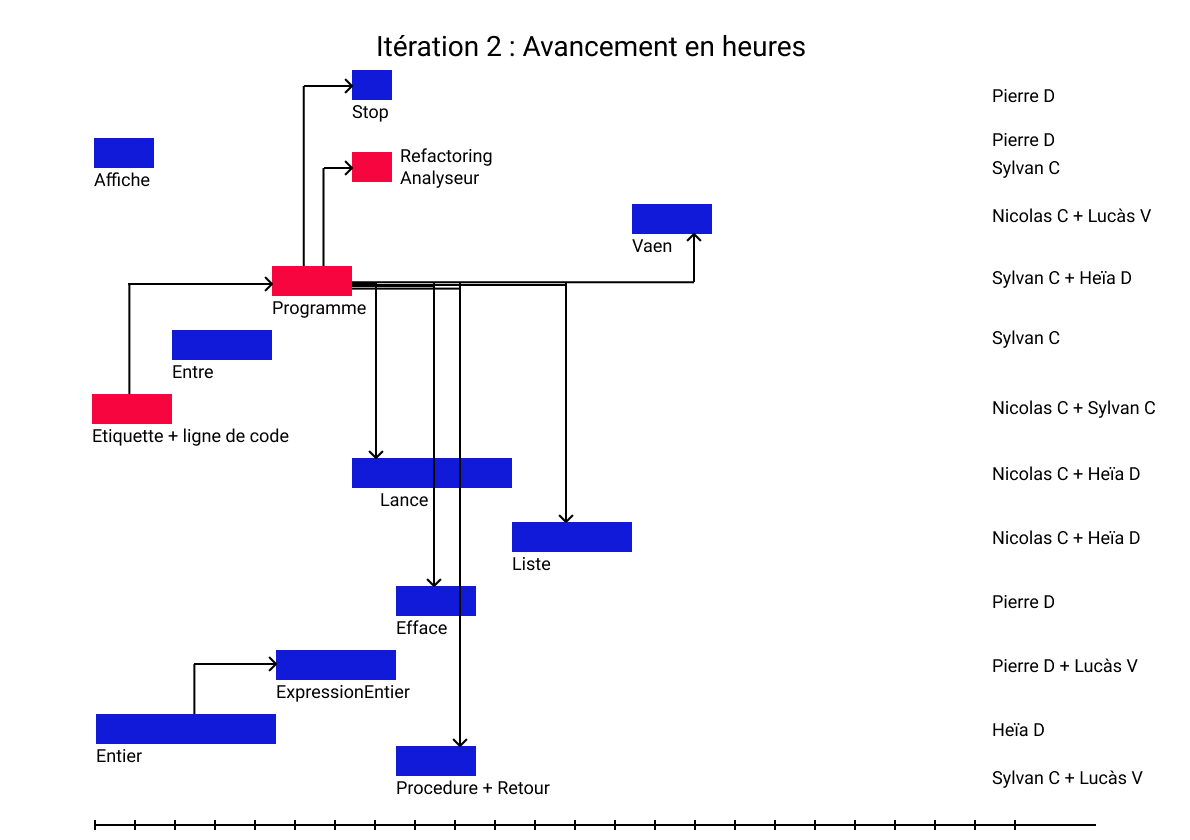
\includegraphics[scale=0.75]{fichiers/planification/iteration2/iteration2Avancement.png}

Au total, la seconde itération aura englobé un temps de travail total de 30,5 heures,
soit 4,5 heures ou 2,25 jours.homme de retard par rapport à la planification initiale. Ce
retard s'explique dans des difficultés à gérer les dépendances avec la classe Programme
et à écrire des tests concluants. Les instructions \verb|lance| et \verb|liste| sont
celles nous ayant posé le plus de problèmes.

Nous pouvons également remarquer, à travers ce graphe, l'étalement dans le temps
des tâches comparé à la planification précédente. Cela est dû à un inconvénient du
travail en binôme. En effet, le nombre de membres de notre équipe étant fini, il nous
a fallu par moments attendre que certains se libèrent d'une tâche pour entamer la
suivante.

En entreprise, cet inconvénient est en général mitigé par la quotité horaire
fixe et convenue dans le contrat de travail. Dans le cadre d'un travail étudiant, nous
avons aussi dû jouer avec les disponibilités de chacun, en plus des contraintes
imposées par le travail à deux. En dépit de ces facteurs, nous n'avons aucun écart
majeur à déplorer dans notre ordonnancement.

%\subsection{Synthèse par "tableau de bord"}

\subsection{Résultats des tests et recette de prototype de la période}

%\subsection{Résultats des revues/suivis/contrôles qualité de la période}

\subsection{Identification des principaux écarts et problèmes constatés, solutions possibles}
\`{A} ce stade du projet, aucun gros écart n'est constaté. Nous avons cependant
été confrontés à des difficultés à mener nos tests correctement, ce qui a fait
augmenter la durée de certaines tâches (non critiques).

\subsection{Propositions de modification de la planification prévisionnelle pour tenir compte des corrections à apporter}

\subsection{Comptes-rendus des réunions projets de la période}

\subsection{Compte-rendu du comité de pilotage de la période}

\subsection{Planification prévisionnelle révisée pour les périodes suivantes (en fonction des décisions prises)}

 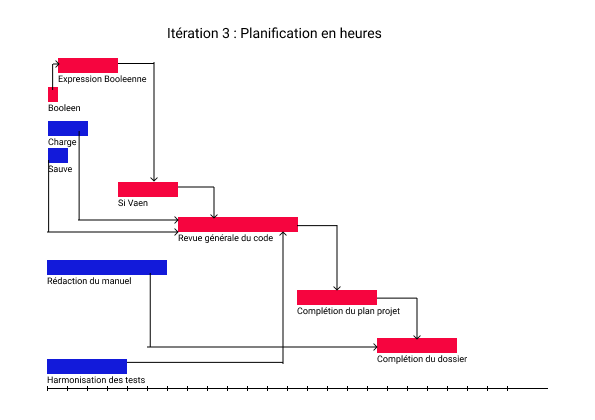
\includegraphics[scale=0.75]{fichiers/planification/iteration3/iteration3Planif.png}

Au vu des estimations effectuées, la troisième itération devrait couvrir un temps
de travail de 33,5 heures, soit 16,75 jours.homme. Cette itération comportant de
nombreuses tâches critiques (le 28 mai marquant le dernier jalon de la phase de
développement et la livraison du prototype final), nous avons délibérément pris des estimations potentiellement larges
afin de nous assurer suffisamment de temps pour mener ces tâches à bien.

\section{Suivi du projet pour la troisième itération}

\subsection{Suivi d’avancement et mesure des écarts par rapport au prévisionnel revu lors de la période précédente}

\subsection{Synthèse par "tableau de bord"}

    \subsection{Résultats des tests et recette de prototype de la période}

\subsection{Résultats des revues/suivis/contrôles qualité de la période}

\subsection{Identification des principaux écarts et problèmes constatés, solutions possibles}

\subsection{Propositions de modification de la planification prévisionnelle pour tenir compte des corrections à apporter}

\subsection{Comptes-rendus des réunions projets de la période}

\subsection{Compte-rendu du comité de pilotage de la période}

\subsection{Planification prévisionnelle révisée pour les périodes suivantes (en fonction des décisions prises)}